\documentclass[11pt,a4paper]{article}

% ============================================================================
% PACKAGES
% ============================================================================
\usepackage[utf8]{inputenc}
\usepackage[T1]{fontenc}
\usepackage{geometry}
\usepackage{graphicx}
\usepackage{booktabs}
\usepackage{amsmath}
\usepackage{amssymb}
\usepackage{hyperref}
\usepackage{xcolor}
\usepackage{listings}
\usepackage{float}
\usepackage{caption}
\usepackage{subcaption}
\usepackage{enumitem}
\usepackage{fancyhdr}
\usepackage{tikz}
\usepackage{pgfplots}
\usepackage{multicol}
\pgfplotsset{compat=1.17}

% ============================================================================
% PAGE SETUP
% ============================================================================
\geometry{margin=1in}
\setlength{\parindent}{0pt}
\setlength{\parskip}{0.5em}

% Header/Footer
\pagestyle{fancy}
\fancyhf{}
\rhead{MetaFam Knowledge Graph}
\lhead{Task 1: Dataset Exploration}
\rfoot{Page \thepage}

% Colors
\definecolor{codegreen}{rgb}{0,0.6,0}
\definecolor{codegray}{rgb}{0.5,0.5,0.5}
\definecolor{codepurple}{rgb}{0.58,0,0.82}
\definecolor{backcolour}{rgb}{0.95,0.95,0.92}

% Hyperref setup
\hypersetup{
    colorlinks=true,
    linkcolor=blue,
    filecolor=magenta,
    urlcolor=cyan,
}

% ============================================================================
% DOCUMENT
% ============================================================================
\begin{document}

% ----------------------------------------------------------------------------
% TITLE PAGE
% ----------------------------------------------------------------------------
\begin{titlepage}
    \centering
    \vspace*{2cm}
    
    {\Huge\bfseries MetaFam Knowledge Graph\\[0.5cm]Task 1: Dataset Exploration\par}
    
    \vspace{1.5cm}
    
    {\Large\textit{``Makes a diff'rence, havin' a decent family''} --- Rubeus Hagrid\par}
    
    \vspace{2cm}
    
    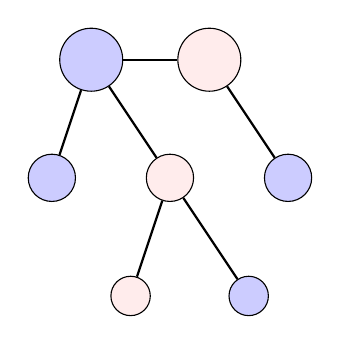
\begin{tikzpicture}
        % Simple family tree illustration
        \node[circle, draw, fill=blue!20, minimum size=0.8cm] (root) at (0,0) {};
        \node[circle, draw, fill=pink!30, minimum size=0.8cm] (sp) at (1.5,0) {};
        \node[circle, draw, fill=blue!20, minimum size=0.6cm] (c1) at (-0.5,-1.5) {};
        \node[circle, draw, fill=pink!30, minimum size=0.6cm] (c2) at (1,-1.5) {};
        \node[circle, draw, fill=blue!20, minimum size=0.6cm] (c3) at (2.5,-1.5) {};
        \node[circle, draw, fill=pink!30, minimum size=0.5cm] (gc1) at (0.5,-3) {};
        \node[circle, draw, fill=blue!20, minimum size=0.5cm] (gc2) at (2,-3) {};
        
        \draw[thick] (root) -- (sp);
        \draw[thick] (root) -- (c1);
        \draw[thick] (root) -- (c2);
        \draw[thick] (sp) -- (c3);
        \draw[thick] (c2) -- (gc1);
        \draw[thick] (c2) -- (gc2);
    \end{tikzpicture}
    
    \vspace{2cm}
    
    {\large Precog Research Task\\[0.3cm]
    Knowledge Graph Analysis on Family Networks\par}
    
    \vfill
    
    {\large February 2026\par}
\end{titlepage}

% ----------------------------------------------------------------------------
% TABLE OF CONTENTS
% ----------------------------------------------------------------------------
\tableofcontents
\newpage

% ----------------------------------------------------------------------------
% SECTION 1: INTRODUCTION
% ----------------------------------------------------------------------------
\section{Introduction}

\subsection{Background}

Knowledge Graphs (KGs) provide a structured representation of real-world entities and their relationships, stored as \textbf{(head, relation, tail)} triples. For example, the triple \texttt{(Alice, motherOf, Bob)} represents that Alice is the mother of Bob, giving textual and semantic meaning to graph structures.

\textbf{MetaFam} is a synthetic family knowledge graph that models familial relationships between individuals. This report presents a comprehensive exploration of the MetaFam dataset, analyzing its structure, computing relevant graph metrics, and extracting qualitative insights about family network organization.

\subsection{Objectives}

The primary objectives of this exploration task are:

\begin{enumerate}[label=\arabic*.]
    \item \textbf{Load and understand} the dataset structure
    \item \textbf{Compute relevant statistics} appropriate for family knowledge graphs
    \item \textbf{Create meaningful visualizations} to support findings
    \item \textbf{Identify important individuals} using graph centrality metrics
    \item \textbf{Understand hierarchical structure} through generational analysis
    \item \textbf{Extract qualitative insights} about family network patterns
\end{enumerate}

\subsection{Theoretical Foundation}

\subsubsection{Graph Representation}

The MetaFam dataset is represented as both:

\begin{itemize}
    \item \textbf{Directed Graph (DiGraph)}: Preserves semantic direction of relationships (e.g., \texttt{fatherOf} implies parent$\rightarrow$child direction). Essential for genealogical analysis.
    \item \textbf{Undirected Graph}: Treats relationships as bidirectional connections. Useful for community detection and clustering analysis.
\end{itemize}

\subsubsection{Why Graph Analysis for Genealogy?}

\begin{itemize}
    \item \textbf{Centrality metrics} identify important individuals (patriarchs, matriarchs)
    \item \textbf{Connected components} reveal separate family lineages
    \item \textbf{Generational depth} maps the family tree hierarchy
    \item \textbf{Clustering coefficient} measures the closure of familial relationships
\end{itemize}

% ----------------------------------------------------------------------------
% SECTION 2: DATASET OVERVIEW
% ----------------------------------------------------------------------------
\section{Dataset Overview}

\subsection{Basic Statistics}

The MetaFam knowledge graph contains the following basic statistics:

\begin{table}[H]
    \centering
    \caption{MetaFam Dataset Summary Statistics}
    \label{tab:basic_stats}
    \begin{tabular}{lrl}
        \toprule
        \textbf{Metric} & \textbf{Value} & \textbf{Description} \\
        \midrule
        Total Nodes (People) & 1,316 & Unique individuals in the graph \\
        Total Edges (Relations) & 13,821 & Family relationship triples \\
        Unique Relationship Types & 28 & Distinct family relation categories \\
        Average Degree & 10.50 & Mean connections per person \\
        \bottomrule
    \end{tabular}
\end{table}

\subsection{Relationship Types}

The 28 unique relationship types in MetaFam can be categorized into six main groups:

\begin{table}[H]
    \centering
    \caption{Relationship Type Categories}
    \label{tab:rel_categories}
    \begin{tabular}{lcp{7cm}}
        \toprule
        \textbf{Category} & \textbf{Count} & \textbf{Relations} \\
        \midrule
        Parent-Child & 12 & fatherOf, motherOf, sonOf, daughterOf, grandfatherOf, grandmotherOf, grandsonOf, granddaughterOf, greatGrandfatherOf, greatGrandmotherOf, greatGrandsonOf, greatGranddaughterOf \\
        \midrule
        Sibling & 2 & brotherOf, sisterOf \\
        \midrule
        Aunt/Uncle & 8 & auntOf, uncleOf, nieceOf, nephewOf, greatAuntOf, greatUncleOf, secondAuntOf, secondUncleOf \\
        \midrule
        Cousin & 6 & boyCousinOf, girlCousinOf, boySecondCousinOf, girlSecondCousinOf, boyFirstCousinOnceRemovedOf, girlFirstCousinOnceRemovedOf \\
        \midrule
        Spouse & 0 & (Not present in dataset) \\
        \bottomrule
    \end{tabular}
\end{table}

\textbf{Key Observation:} The absence of spouse relations (\texttt{husbandOf}, \texttt{wifeOf}) in the dataset is notable. This suggests the graph focuses on blood relations rather than marriage connections, which has implications for link prediction tasks.

% ----------------------------------------------------------------------------
% SECTION 3: STRUCTURAL ANALYSIS
% ----------------------------------------------------------------------------
\section{Structural Analysis}

\subsection{Global Network Metrics}

\subsubsection{Graph Density}

\begin{equation}
    \text{Density} = \frac{|E|}{|V| \times (|V| - 1)} = \frac{13,821}{1,316 \times 1,315} = 0.007987
\end{equation}

The graph density of \textbf{0.008} indicates a \textbf{very sparse network}, which is characteristic of social and family networks. This sparsity arises because each individual connects only to a limited set of relatives, not to everyone in the extended family network.

\textbf{Interpretation:} In a family network, even with 1,316 people, each person only has direct relationships with approximately 10-11 others on average, resulting in the observed sparse connectivity pattern.

\subsubsection{Clustering Coefficient}

\begin{equation}
    \text{Average Clustering Coefficient} = 0.7346
\end{equation}

The \textbf{high clustering coefficient (0.73)} indicates strong transitivity in family relationships. This means:

\begin{itemize}
    \item If person A is related to B, and B is related to C, there's a high probability A is also related to C
    \item Family structures naturally form tight-knit clusters
    \item Siblings share parents, cousins share grandparents, etc.
\end{itemize}

\subsection{Connectivity Analysis}

\begin{table}[H]
    \centering
    \caption{Connected Component Statistics}
    \label{tab:connectivity}
    \begin{tabular}{lr}
        \toprule
        \textbf{Metric} & \textbf{Value} \\
        \midrule
        Weakly Connected Components & 50 \\
        Largest Component Size & 27 nodes \\
        Smallest Component Size & 26 nodes \\
        Average Component Size & 26.3 nodes \\
        \bottomrule
    \end{tabular}
\end{table}

\textbf{Key Insights:}

\begin{enumerate}
    \item \textbf{Forest Structure:} The graph is a \textbf{forest} consisting of 50 separate family trees, not a single connected component.
    
    \item \textbf{Uniform Family Sizes:} Component sizes are remarkably uniform (26-27 nodes), suggesting synthetically generated families of similar structure.
    
    \item \textbf{No Bridges Between Families:} The absence of spouse relations means families remain isolated---in real genealogy, marriages would create bridges between family clusters.
\end{enumerate}

\subsection{Degree Distribution}

\begin{table}[H]
    \centering
    \caption{Degree Statistics}
    \label{tab:degree}
    \begin{tabular}{lccc}
        \toprule
        \textbf{Metric} & \textbf{Min} & \textbf{Max} & \textbf{Mean} \\
        \midrule
        In-Degree & 0 & 23 & 10.50 \\
        Out-Degree & 1 & 22 & 10.50 \\
        \bottomrule
    \end{tabular}
\end{table}

\textbf{Asymmetry Analysis:}

In directed family knowledge graphs with relations like \texttt{fatherOf}:
\begin{itemize}
    \item \textbf{High Out-Degree}: Indicates ancestors (they have many \texttt{parentOf}, \texttt{grandparentOf} relations pointing out)
    \item \textbf{High In-Degree}: Indicates individuals with many relations pointing TO them (heavily referenced)
\end{itemize}

% ----------------------------------------------------------------------------
% SECTION 4: GENERATIONAL ANALYSIS
% ----------------------------------------------------------------------------
\section{Generational Analysis}

\subsection{Generation Computation Algorithm}

Generational depth is computed using a BFS-based algorithm:

\begin{enumerate}
    \item Extract parental subgraph (only \texttt{fatherOf}, \texttt{motherOf} edges)
    \item Identify root nodes (in-degree = 0 in parental subgraph)
    \item Run BFS from roots, assigning generation levels
    \item Handle disconnected components separately
\end{enumerate}

\subsection{Generation Distribution}

\begin{table}[H]
    \centering
    \caption{Generation Distribution in MetaFam}
    \label{tab:generation}
    \begin{tabular}{crr}
        \toprule
        \textbf{Generation} & \textbf{Count} & \textbf{Percentage} \\
        \midrule
        Generation 0 (Great-grandparents) & 519 & 39.4\% \\
        Generation 1 (Grandparents) & 572 & 43.5\% \\
        Generation 2 (Parents) & 216 & 16.4\% \\
        Generation 3 (Children) & 9 & 0.7\% \\
        \midrule
        \textbf{Total} & \textbf{1,316} & \textbf{100\%} \\
        \bottomrule
    \end{tabular}
\end{table}

\textbf{Key Insights:}

\begin{enumerate}
    \item \textbf{4 Generations}: The family graph spans 4 generations (0-3), representing great-grandparents through great-grandchildren.
    
    \item \textbf{Inverted Pyramid}: Newer generations (Gen 2, 3) have significantly fewer members, reflecting typical family tree structures where older generations have more accumulated members over time.
    
    \item \textbf{Mean Generation = 0.78}: The average person is in an early generation, consistent with the pyramid structure.
    
    \item \textbf{Few Youngest Members}: Only 9 individuals (0.7\%) are in Generation 3, the most recent generation.
\end{enumerate}

\subsection{Generational Relevance for Link Prediction}

Generation information is crucial for predicting relationships:
\begin{itemize}
    \item \texttt{fatherOf} relations only occur from Gen $n$ to Gen $n+1$
    \item \texttt{grandparentOf} relations span two generations
    \item \texttt{siblingOf} relations occur within the same generation
    \item \texttt{cousinOf} relations exist between individuals of similar generations in different branches
\end{itemize}

% ----------------------------------------------------------------------------
% SECTION 5: GENDER ANALYSIS
% ----------------------------------------------------------------------------
\section{Gender Classification}

\subsection{Rule-Based Inference}

Gender is inferred deterministically based on relationship semantics where a node appears as the \textbf{HEAD} (source) of a relation:

\textbf{Male-indicating relations:}
\begin{verbatim}
fatherOf, brotherOf, sonOf, uncleOf, grandfatherOf,
nephewOf, boyCousinOf, grandsonOf, greatUncleOf, ...
\end{verbatim}

\textbf{Female-indicating relations:}
\begin{verbatim}
motherOf, sisterOf, daughterOf, auntOf, grandmotherOf,
nieceOf, girlCousinOf, granddaughterOf, greatAuntOf, ...
\end{verbatim}

\subsection{Gender Distribution}

\begin{table}[H]
    \centering
    \caption{Gender Distribution}
    \label{tab:gender}
    \begin{tabular}{lrr}
        \toprule
        \textbf{Gender} & \textbf{Count} & \textbf{Percentage} \\
        \midrule
        Female & 670 & 50.9\% \\
        Male & 646 & 49.1\% \\
        Unknown & 0 & 0\% \\
        Unmapped (conflicts) & 0 & 0\% \\
        \midrule
        \textbf{Total} & \textbf{1,316} & \textbf{100\%} \\
        \bottomrule
    \end{tabular}
\end{table}

\textbf{Key Insights:}

\begin{enumerate}
    \item \textbf{Balanced Distribution}: Near-perfect gender balance (51\% female, 49\% male)
    
    \item \textbf{Complete Classification}: 100\% of nodes successfully classified (no unknowns or conflicts)
    
    \item \textbf{Data Quality}: Zero unmapped nodes indicates no data inconsistencies (no individual assigned conflicting gender-based relations)
    
    \item \textbf{Link Prediction Utility}: Gender is a strong constraint for predicting gender-specific relations (\texttt{brotherOf} vs \texttt{sisterOf})
\end{enumerate}

% ----------------------------------------------------------------------------
% SECTION 6: CENTRALITY ANALYSIS
% ----------------------------------------------------------------------------
\section{Centrality Analysis}

\subsection{PageRank Centrality}

PageRank measures node importance based on the quality of incoming connections:

\begin{equation}
    PR(v) = \frac{1-d}{N} + d \sum_{u \rightarrow v} \frac{PR(u)}{out(u)}
\end{equation}

where $d = 0.85$ (damping factor) and $N$ = number of nodes.

\begin{table}[H]
    \centering
    \caption{PageRank Statistics}
    \label{tab:pagerank_stats}
    \begin{tabular}{lr}
        \toprule
        \textbf{Metric} & \textbf{Value} \\
        \midrule
        Minimum & 0.000114 \\
        Maximum & 0.001857 \\
        Mean & 0.000760 \\
        \bottomrule
    \end{tabular}
\end{table}

\subsubsection{Top Individuals by PageRank}

\begin{table}[H]
    \centering
    \caption{Top 10 Individuals by PageRank (``Important Ancestors'')}
    \label{tab:top_pagerank}
    \begin{tabular}{clcc}
        \toprule
        \textbf{Rank} & \textbf{Node} & \textbf{PageRank} & \textbf{Generation} \\
        \midrule
        1 & gabriel241 & 0.001857 & 2 \\
        2 & lea1165 & 0.001841 & 2 \\
        3 & raphael29 & 0.001809 & 2 \\
        4 & christian712 & 0.001682 & 2 \\
        5 & tobias713 & 0.001682 & 2 \\
        6 & emilia428 & 0.001676 & 2 \\
        7 & simon172 & 0.001644 & 2 \\
        8 & victoria279 & 0.001631 & 2 \\
        9 & benjamin952 & 0.001603 & 1 \\
        10 & helena1135 & 0.001571 & 2 \\
        \bottomrule
    \end{tabular}
\end{table}

\textbf{Observation:} Most high-PageRank individuals are in Generation 2, indicating they are ``important ancestors'' with many descendants pointing to them through various relationships.

\subsection{Betweenness Centrality}

Betweenness centrality measures how often a node lies on shortest paths:

\begin{equation}
    B(v) = \sum_{s \neq v \neq t} \frac{\sigma_{st}(v)}{\sigma_{st}}
\end{equation}

\begin{table}[H]
    \centering
    \caption{Top 5 ``Bridge'' Individuals by Betweenness}
    \label{tab:top_betweenness}
    \begin{tabular}{clc}
        \toprule
        \textbf{Rank} & \textbf{Node} & \textbf{Betweenness} \\
        \midrule
        1 & lea1165 & 0.0001 \\
        2 & valentin638 & 0.0001 \\
        3 & gabriel241 & 0.0001 \\
        4 & nora536 & 0.0001 \\
        5 & stefan1192 & 0.0001 \\
        \bottomrule
    \end{tabular}
\end{table}

\textbf{Key Insight:} Betweenness centrality values are very low (max = 0.0001), indicating \textbf{few bridge individuals} in the network. This is consistent with the forest structure---without inter-family marriages, there are no natural bridges connecting different family clusters.

\subsection{Degree-Based Importance}

\subsubsection{Top by Out-Degree (Ancestors)}

\begin{table}[H]
    \centering
    \caption{Top 5 Individuals by Out-Degree}
    \label{tab:top_outdegree}
    \begin{tabular}{clcc}
        \toprule
        \textbf{Rank} & \textbf{Node} & \textbf{Out-Degree} & \textbf{Generation} \\
        \midrule
        1 & oskar133 & 22 & 2 \\
        2 & larissa136 & 22 & 2 \\
        3 & fabian140 & 22 & 2 \\
        4 & laura143 & 22 & 2 \\
        5 & dominik1036 & 22 & 2 \\
        \bottomrule
    \end{tabular}
\end{table}

High out-degree indicates many outgoing relations (\texttt{parentOf}, \texttt{grandparentOf}), identifying \textbf{prolific ancestors}.

% ----------------------------------------------------------------------------
% SECTION 7: QUALITATIVE INSIGHTS
% ----------------------------------------------------------------------------
\section{Qualitative Insights}

\subsection{Structural Characteristics}

\begin{enumerate}
    \item \textbf{Sparse Graph}: Family knowledge graphs are inherently sparse ($\text{density} < 0.01$) because individuals only connect to immediate and extended family, not the entire population.
    
    \item \textbf{No Self-Loops}: The graph contains no self-loops (a person cannot be their own relative), which is domain-appropriate.
    
    \item \textbf{Forest Structure}: The graph is a forest of 50 disjoint family trees. In real genealogy, marriages would create bridges, but this synthetic dataset lacks spouse relations.
    
    \item \textbf{Directed Edges}: Edge direction encodes semantic meaning (parent$\rightarrow$child vs child$\rightarrow$parent).
\end{enumerate}

\subsection{Implications for Downstream Tasks}

\subsubsection{Community Detection (Task 2)}
\begin{itemize}
    \item Each connected component is already a natural ``community'' (family unit)
    \item Within families, sub-communities may correspond to nuclear family units
    \item Generation boundaries may define community structure
\end{itemize}

\subsubsection{Rule Mining (Task 3)}
\begin{itemize}
    \item Transitive rules: $(X, \text{fatherOf}, Y) \land (Y, \text{fatherOf}, Z) \rightarrow (X, \text{grandfatherOf}, Z)$
    \item Inverse rules: $(X, \text{fatherOf}, Y) \rightarrow (Y, \text{sonOf}, X)$
    \item Gender constraints: $(X, \text{motherOf}, Y) \rightarrow \text{gender}(X) = \text{Female}$
\end{itemize}

\subsubsection{Link Prediction (Task 4)}
Node attributes are valuable features:
\begin{itemize}
    \item \textbf{Generation}: Constrains relation types (parent-child spans 1 gen, grandparent spans 2)
    \item \textbf{Gender}: Determines gender-specific relations (\texttt{brotherOf} vs \texttt{sisterOf})
    \item \textbf{Community}: Relationships more likely within the same family cluster
    \item \textbf{PageRank}: High-PageRank nodes more likely to have additional links
    \item \textbf{Degree}: Highly connected individuals have more potential for additional links
\end{itemize}

% ----------------------------------------------------------------------------
% SECTION 8: NODE ATTRIBUTES
% ----------------------------------------------------------------------------
\section{Node Attributes for Export}

The following attributes are computed and stored for each node, exported to GEXF format for Gephi visualization:

\begin{table}[H]
    \centering
    \caption{Node Attributes Stored in Graph}
    \label{tab:node_attrs}
    \begin{tabular}{llp{7cm}}
        \toprule
        \textbf{Attribute} & \textbf{Type} & \textbf{Description} \\
        \midrule
        \texttt{in\_degree} & int & Number of incoming edges \\
        \texttt{out\_degree} & int & Number of outgoing edges \\
        \texttt{pagerank} & float & PageRank centrality score (0-1) \\
        \texttt{generation} & int & Generational depth (0 = oldest, -1 = unassigned) \\
        \texttt{gender} & str & Male / Female / Unknown / Unmapped \\
        \bottomrule
    \end{tabular}
\end{table}

\textbf{Note:} Betweenness centrality is computed for analysis but \textbf{not stored} as a node attribute.

\subsection{Gephi Visualization Recommendations}

\begin{enumerate}
    \item \textbf{Color nodes by}: \texttt{gender} attribute (blue = male, pink = female)
    \item \textbf{Size nodes by}: \texttt{pagerank} or \texttt{out\_degree}
    \item \textbf{Vertical layout}: Use \texttt{generation} for Y-axis positioning
    \item \textbf{Layout algorithm}: ForceAtlas2 works well for family tree visualization
\end{enumerate}

% ----------------------------------------------------------------------------
% SECTION 9: SUMMARY
% ----------------------------------------------------------------------------
\section{Summary}

\subsection{Key Findings}

\begin{table}[H]
    \centering
    \caption{Summary of Key Findings}
    \label{tab:summary}
    \begin{tabular}{p{5cm}p{8cm}}
        \toprule
        \textbf{Aspect} & \textbf{Finding} \\
        \midrule
        \textbf{Scale} & 1,316 people, 13,821 relations, 28 relation types \\
        \textbf{Structure} & Forest of 50 families, ~26-27 members each \\
        \textbf{Sparsity} & Density = 0.008 (typical for social networks) \\
        \textbf{Clustering} & High transitivity (0.73) due to family structure \\
        \textbf{Depth} & 4 generations, pyramid distribution \\
        \textbf{Gender} & Balanced (51\% F, 49\% M), fully classified \\
        \textbf{Central Figures} & Identified via PageRank, mostly Gen 2 ancestors \\
        \bottomrule
    \end{tabular}
\end{table}

\subsection{Output Files}

\begin{itemize}
    \item \texttt{outputs/gephi/metafam\_task1\_refined.gexf} --- Enriched graph for Gephi
    \item \texttt{outputs/plots/relationship\_distribution.png} --- Bar chart of relation frequencies
    \item \texttt{outputs/plots/degree\_distribution.png} --- In/out degree histograms
    \item \texttt{outputs/plots/generation\_distribution.png} --- Generation histogram
    \item \texttt{outputs/plots/gender\_distribution.png} --- Gender bar chart
\end{itemize}

% ----------------------------------------------------------------------------
% APPENDIX
% ----------------------------------------------------------------------------
\appendix
\section{Complete Relationship List}

\begin{multicols}{2}
\begin{enumerate}[label=\arabic*.]
    \item auntOf
    \item boyCousinOf
    \item boyFirstCousinOnceRemovedOf
    \item boySecondCousinOf
    \item brotherOf
    \item daughterOf
    \item fatherOf
    \item girlCousinOf
    \item girlFirstCousinOnceRemovedOf
    \item girlSecondCousinOf
    \item granddaughterOf
    \item grandfatherOf
    \item grandmotherOf
    \item grandsonOf
    \item greatAuntOf
    \item greatGranddaughterOf
    \item greatGrandfatherOf
    \item greatGrandmotherOf
    \item greatGrandsonOf
    \item greatUncleOf
    \item motherOf
    \item nephewOf
    \item nieceOf
    \item secondAuntOf
    \item secondUncleOf
    \item sisterOf
    \item sonOf
    \item uncleOf
\end{enumerate}
\end{multicols}

\section{Theoretical Formulas Reference}

\subsection{Graph Density}
For a directed graph $G = (V, E)$:
\begin{equation}
    D = \frac{|E|}{|V| \cdot (|V| - 1)}
\end{equation}

\subsection{Clustering Coefficient}
For node $v$ with neighbors $N(v)$:
\begin{equation}
    C(v) = \frac{|\{e_{jk} : v_j, v_k \in N(v), e_{jk} \in E\}|}{|N(v)| \cdot (|N(v)| - 1)}
\end{equation}

\subsection{PageRank}
Iterative formula with damping factor $d = 0.85$:
\begin{equation}
    PR(v) = \frac{1-d}{N} + d \sum_{u \in B(v)} \frac{PR(u)}{L(u)}
\end{equation}
where $B(v)$ is the set of nodes linking to $v$, and $L(u)$ is the out-degree of $u$.

\subsection{Betweenness Centrality}
\begin{equation}
    B(v) = \sum_{s \neq v \neq t \in V} \frac{\sigma_{st}(v)}{\sigma_{st}}
\end{equation}
where $\sigma_{st}$ is the number of shortest paths from $s$ to $t$, and $\sigma_{st}(v)$ is the number passing through $v$.

\end{document}
